%\documentclass[twocolumn,nofootinbib]{revtex4}
\documentclass[nofootinbib]{revtex4}
%\usepackage{amsmath}
%\usepackage{iopams}
\usepackage{amsmath}
\usepackage{hyperref}
\usepackage{amssymb}
\usepackage{color}
\usepackage{epsfig}
\usepackage{latexsym}
\usepackage{tensor}
%\usepackage{wasysym}
\usepackage{comment}
%\usepackage{graphicx}
%\usepackage{psfrag}


\newcommand{\gw}{gravitational wave }
\newcommand{\gws}{gravitational waves }
\newcommand{\subgw}{_{\textrm{\scriptsize{GW}}}}
\newcommand{\ee}[1]{\!\times\!10^{#1}}
\newcommand{\prob}{{\rm Pr}}
\newcommand{\grbrate}{{{\mathcal R}_{\mathrm{grb}}}}
\newcommand{\cbcrate}{{{\mathcal R}}}
\newcommand{\diff}{{\mathrm d}}
\newcommand{\rhostar}{{\rho^*}}

\begin{document}

\title{Constraints On Short, Hard Gamma-Ray Burst Beaming Angles From
Gravitational Wave Observations}
\author{James Clark, Ik Siong Heng, Martin Hendry}
\date{\today}

\begin{abstract}
Apologies in advance for inconsistent conditioning statements in probabilities
\dots
\end{abstract}

\maketitle

\tableofcontents

\section{Introduction}

It is common in the literature to draw inferences on the rate of binary
coalescence $\cbcrate$, given some estimate for the beaming angle $\theta$ and
the observed rate of sGRBs $\grbrate$.  In this work, we investigate what
statements can \emph{currently} be made on the beaming angle itself using the
upper limits placed on $\cbcrate$ from all-sky, all-time \gw searches and
explore the potential for direct inference of sGRB  beaming angles in the
advanced detector era.

%\section{Limits On sGRB Beaming Angles From Past Gravitational Wave Searches}
\section{Inferring The sGRB Beaming Angle From Rate Measurements}
Assuming that at least some fraction of sGRBs are due to compact binary
coalescence, the observed rate of sGRBs may be written,
%
\begin{equation}\label{eq:rate2angle}
\grbrate=\epsilon\cbcrate(1-\cos \theta),
\end{equation}
%
where $\cbcrate$ is the rate of binary coalescence, $\theta$ is the beaming
angle of the outflow from the GRB and $\epsilon$ is the (generally unknown)
probability that a binary coalescence results in an observed sGRB.  In this
work, we assume
$\grbrate=10$\,Gpc$^{-3}$\,yr$^{-1}$~\cite{nakar-2007,Dietz11}.
 
Inferences of the GRB beaming angle are made from the posterior probability
density on the beaming angle $p(\theta|D,I)$.  Our goal then, is to transform
the measured posterior probability density on the rate $\cbcrate$ to a posterior
on the beaming angle.
%
First, note that the PDF $p(\theta|D,I)$ may be written as a marginalisation
over $\epsilon$ in the the joint PDF $p(\theta, \epsilon|D,I)$:
%
\begin{equation}
p(\theta) = \int_{\epsilon} p(\theta,\epsilon)~\diff \epsilon,
\end{equation}
%
where we have dropped the conditioning statements temporarily for notational
convenience.  Next, we note that the joint probability $p(\theta,\cbcrate)$ can
be written in terms of $\epsilon$ and $\cbcrate$ according to,
%
\begin{equation}
p(\theta,\epsilon) = p(\cbcrate,\epsilon)
\left\lvert\left\lvert
\frac{\partial(\cbcrate,\epsilon)}{\partial(\theta,\epsilon)}
\right\rvert\right\rvert,
\end{equation}
%
where the Jacobian matrix is given by,
% Increase matrix line spacing
\begingroup
\renewcommand*{\arraystretch}{1.5}

% matrix:
\begin{equation}
\frac{\partial (\cbcrate,\epsilon)}{\partial(\theta,\epsilon)} =
\begin{bmatrix}
\frac{\partial \cbcrate}{\partial \theta} & \frac{\partial \cbcrate}{\partial \epsilon} \\
\frac{\partial \epsilon}{\partial \theta} & \frac{\partial \epsilon}{\partial \epsilon}
\end{bmatrix}.
\end{equation}

% end line spacing increase
\endgroup
%%
Bringing all of these terms together then, and writing out the Jacobian matrix
determinant, we have
%
\begin{equation}\label{eq:marginaltheta}
p(\theta) = \frac{2\grbrate \sin
\theta}{(\cos\theta-1)^2}\int_{\epsilon} \frac{p(\epsilon)p(\cbcrate)}{\epsilon} ~\diff
\epsilon,
\end{equation}
%
where we have assumed $\epsilon$ and $\cbcrate$ are logically independent such
that,
\begin{equation}
p(\epsilon,\cbcrate) = p(\epsilon|\cbcrate)p(\cbcrate) = p(\epsilon)p(\cbcrate).
\end{equation}
%
%
To find the target PDF $p(\theta|D,I)$ then, we require the measured coalescence
rate posterior $p(\cbcrate|D,I)$, and we must specify a prior PDF for $\epsilon$
which encapsulates assumptions made about the relative rates of compact binary
mergers and sGRBs.
 
Following~\cite{Biswas09,BradyFairhurst08}, the posterior on the binary
coalescence rate may be determined from the loudest event in the \gw
analysis.  Specifically, for a foreground event rate due to  binary coalescence
$\cbcrate$, the probability of obtaning no events with ranking statistic $\rho$
greater than the observed loudested event $\rhostar$ is,
%
\begin{equation}
P_F(\rhostar | \cbcrate, C_L, T) = e^{-\cbcrate C_L(\rhostar) T},
\end{equation}
%
where $C_L(\rhostar)$ is the total luminosity to which the search is sensitive
and $T$ is the duration of the search.  The overall probability of obtaining
no events with ranking statistic $\rho>\rhostar$ is the product of obtaining
no such events from foreground \emph{and} the probability of obtaining no such
events from the background in the detector, denoted $P_B(\rhostar)$,
%
\begin{equation}
P(\rhostar|\cbcrate,I) = P_B(\rhostar|I)e^{-\cbcrate C_L(\rhostar) T}
\end{equation}
%
Using a uniform prior on $\cbcrate$ and inverting the overall probability with
Bayes' theorem, we arrive at,
%
\begin{equation}\label{eq:loudestEventPosterior}
p(\cbcrate | C_L({\rhostar}, T, \Lambda) \propto p(\cbcrate) \left[ \frac{1+\Lambda
C_L(\rhostar) T}{1+\Lambda}\right] e^{-\cbcrate C_L(\rhostar) T}
\end{equation}
%
where $p(\cbcrate)$ is the prior probability distribution on the rate.  The
quantity $\hat{\Lambda}$ measures the relative probability of detecting an event
with ranking statistic $x$ due to \gws versus the probability of an equally loud
event arising in the background distribution.  The reader is directed to
section\,3 of~\cite{BradyFairhurst08} for a full discussion of this quantity.

%
%\subsection{Incomplete Sky-Coverage \& Unknown GRB Rate}
%Marginalise over some stuff for the case of an `impure' GRB sample (unknown
%fraction of CBCs).
%\\

\section{Beaming Angle Limits From Past GW Searches}

In this section, we focus attention on the interpretation of rate upper limits
from past \gw analyses.  We first reconstruct the measured posterior on the
binary coalescence rate and go on to compute the posterior and upper limit on
the sGRB beaming angle under a range of assumptions regarding the sGRB
efficiency $\epsilon$.

The upper limit on the binary coalescence rate at confidence $\alpha$ is found
by integrating the rate posterior from zero to $\alpha$.  Assuming a uniform
prior on the rate $\cbcrate$ and using the rate posterior given by
equation~\ref{eq:loudestEventPosterior}, the upper limit on the rate
$\cbcrate_{\alpha}$ is given by equation 21 in~\cite{BradyFairhurst08}:
%
\begin{equation}
1-\alpha =  e^{-\cbcrate_{\alpha} C_L(\rhostar)T)}
\left[ 
1+ \left(\frac{\Lambda}{1+\Lambda}\right) \cbcrate_{\alpha} T C_L(\rhostar)
\right ].
\label{eq:rateIntegral}
\end{equation}
%
In the event that no \gw signal has been observed and the loudest event is
umabiguously due to background noise fluctuations, we are in the limit in which
$\Lambda \rightarrow 0$.  In this case, we simply have,
\begin{equation}
C_L(\rhostar)T = -\frac{\log(1-\alpha)}{\cbcrate_{\alpha}},
\end{equation}
%
and the value of $\cbcrate$ can be taken straight from the literature\footnote{Note
that this procedure necessarily confines our jet angle inferences based on
progenitor systems for which the rate upper limits are available.  Given that
the binary coalesence rate limits are quoted for canonical binary neutron star
and neutron star-black hole systems, both plausible sGRB progenitors, this
simply means our inferences on the jet angle are specific to each system and
treated separately.}

Using the most stringent 90\% confidence upper limit from \gw observations on
the rate of binary neutron star coalescences to date, $\cbcrate^{90\%}_{{\rm
bns}} = 1.3\times 10^{-4}$\,Mpc$^{-3}$yr$^{-1}$~\cite{S6lowmass}, gives
$C_L(\rhostar)T=17712$.  Similarly, for NS-BH systems,  $\cbcrate^{90\%}_{{\rm
nsbh}} = 3.1\times 10^{-5}$\,Mpc$^{-3}$yr$^{-1}$ gives $C_L(\rhostar)T=74277$.
The posteriors on the rates, assuming these values and $\Lambda=0$, are shown in
figure~\ref{fig:reconstructedRatePosterior}.  

\begin{figure}
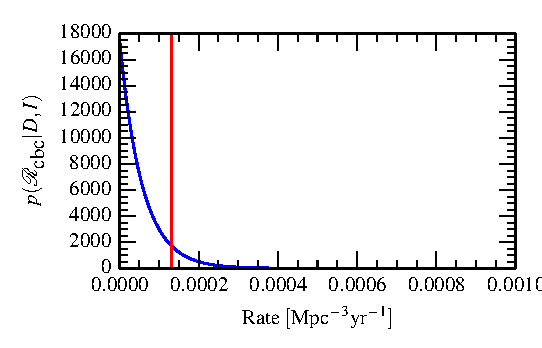
\includegraphics{rate_posterior_s6UL_TEST_deltaEffPrior-1.0.eps}
\caption{Rate posterior for S6/VSR2,3 Low-mass Search For Compact Binary
Coalescence.\label{fig:reconstructedRatePosterior}}
\end{figure}

\subsection{Known GRB Efficiency, $\epsilon$}

Figure~\ref{fig:jetPosterior} shows the resulting posterior on the GRB
beaming angle, using the transformation in equation~\ref{eq:rate2angleProb} and
our results so far.  
%
Now, the quantity of interest is the upper limit on the jet
angle~$\theta^{90\%}$:
%
\begin{equation}
0.9 = \int_{\theta^{90\%}}^{\infty}p(\theta | \cbcrate^{90\%})~\diff \theta
\end{equation}
%
This is indicated with the vertical red line in figure~\ref{fig:jetPosterior}.
We find $\theta^{90\%}=3.3^{\circ}$.


\begin{figure}
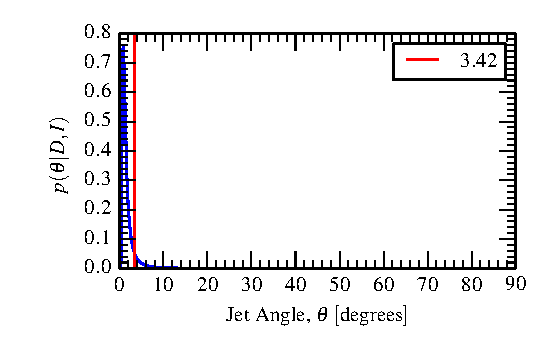
\includegraphics{jet_angle_posterior_s6UL_TEST_deltaEffPrior-1.0.eps}
\caption{Jet angle posterior derived from S6/VSR2,3 Low-mass Search For Compact Binary
Coalescence posterior / upper limit on compact binary coalescence
rate, assuming \emph{all} BNS result in sGRBs.\label{fig:jetPosterior}}
\end{figure}


\subsection{Unknown GRB Efficiency, $\epsilon$}


\subsection{Astrophysical Interpretation \& Comparison With Other Limits}
The comparison with other limits is straightforward.  I think it looks pretty
consistent with Dietz, Holtz etc (but should double check).

More importantly, however,  we've demonstrated how to get a limit on the beaming
angle.  That's all well and good but we need some astrophysical interpretation,
really.  The most obvious thing (to James) is that the beaming angle is really a
proxy for the Lorentz factor of the outflow (I think):
%
\begin{equation}
\theta \sim \frac{1}{\Gamma}.
\end{equation}
%
So, what \emph{physics} of the progenitor can we constrain with this?

\section{Beaming Angle Inferences In The Detection Era}
In this section, we discuss an approach to measuring the GRB beaming angle based
on the binary coalescence rate as measured from a pair of detection scenarios.
In the first instance, we consider an imagined `early' science run with the the
advanced LIGO detectors where ${\mathcal O}(1)$ gravitational wave events from
binary neutron star coalescence are detected.  In the second secnario, we
consider the measurements possible with multiple gravitational wave detections.
\textcolor{red}{This section will draw heavily on the observing scenarios
section (4) in~\cite{ade_prospects}.}

\subsection{For discussion: Post-detection Coalescence Rate Posterior}
Here, we determine the formalism for the construction of a rate
posterior in the event of single or multiple gravitational wave detections.
%
There needs to be no specific discussion of GRBs here, it's more general than
that.  In fact, it's worth remembering \emph{nothing} in this paper / analysis
(so far) has assumed contemporaneous GRB-GW detections!\footnote{although that
does seem like a potential avenue for measuring the CBC-sGRB efficiency \dots}.
All we actually do is assume we have independent measurements of BNS and sGRB
rates.

\textcolor{red}{Rather, the point of this discussion is to determine/describe
a simple, natural way to construct the posterior on the rate $\cbcrate$, given
multiple GW detections}, as expected in the advanced detector era.

Recall the rate posterior from Fairhurst \& Brady~\cite{BradyFairhurst08}:
\begin{equation}\label{eq:full_ratePosterior}
p(\cbcrate|\rho_m, T, B) \propto p(R) \left[ \frac{1+\Lambda R
C_L(\rho_m)T}{1+\Lambda} e^{-RC_L(\rho_m)T}\right]
\end{equation}
%
Equation~\ref{eq:full_ratePosterior} is the posterior on the rate, as measured
by the single loudest event in the search conducted.  In the equation above,
$\Lambda$ is the likelihood of the \emph{loudest event} being from GW vs
background and $C_L$ is the cumulative luminosity the search which produced
loudest event $\rho_m$ is sensitive to.  It's a neat, sensible approach to
estimating event rates given very rare measurements.  That is, it seems like a
Good Thing / natural for constructing a rate posterior where we only expect a
single signal trigger from a population of potentially trigger-inducing events.
It also seems sensible:
%
\begin{itemize}
\item in the absence of convincing detections (loudest event is unlikely to be a
signal; $\Lambda \rightarrow 0$),
\item for a single, convincing detection (loudest event is very likely to be a
signal; $\Lambda \rightarrow \infty$).
\end{itemize}
%
It's worth highlighting here that there is absolutely nothing \emph{preventing}
one from using the loudest event statistic when we expect more than one signal
trigger; regardless of how many events we have, there's always going be a
loudest one and we can always determine the probability of obtaining a trigger
that loud, given the sensitivity of the search and a population model.  Indeed,
consider the key components in the ocnstruction of the L.E. posterior:
%
\begin{enumerate}
\item The loudest event, characterised by, say, single IFO signal-to-noise ratio
$\rho$.  Label this loudest value $\rho_m$.
\item The probability of obtaining zero events with $\rho>\rho_m$ from a
population of signals; this is formed from knowledge of the sensitivity of the
analysis and a population model.  It does not require that there be only a
single signal observed in the experiment.
\item The probability of obtaining zero events with $\rho>\rho_m$, from a
population of background fluctuations (Gaussian or otherwise).
\end{enumerate}
%
The (potential) issue at hand is the following: suppose the most
optimistic rate estimates are correct and aLIGO instantaneously reaches full
design sensitivity.  In one year, we will have acquired ${\mathcal O}(100)$ BNS
detections.  That's an entire year of measurements and a sizeable population of
SNR measurements.  Here's the big question: 
\begin{quote}
{\bf \textcolor{red}{If we form the rate
posterior from the loudest event, are we in any sense `throwing away'
information by considering only the loudest trigger?}}
\end{quote}
Equally importantly (and, at the risk of sounding glib, not necessarily the same
point\dots):
\begin{quote}
{\bf \textcolor{red}{Does the L.E. formalism reflect what we'll actually do
with, say, 100 BNS detections in aLIGO?}}
\end{quote}

Without thinking about it too hard, it `feels' like we're literally throwing
away 99\% of the information gathered in the experiment.  But is that true?
That is, if we use the observation time of the experiment together with an
estimate of the distance / volume sensitivity of the search, is there actually
any more information to be gleaned from a sample of GW triggers than is already
present in the value of the loudest trigger?  Is it perhaps the case that the
loudest event probes the \emph{tail} of the SNR distribution, while a sample
of triggers allows one to better estimate the full distribution of SNRs?

\subsection{Alternative Rate Posterior Construction From \S 14 in Gregory}
Gregory's book, `Logical Data Analysis For The Physical Sciences' has an entire
chapter (\S 14) devoted to `Bayesian Inference With Poisson Sampling'.  This
seems to match our problem rather well.  In particular, he derives expressions
for a Poisson rate posterior in \S 14.3, `Signal + known background' and, even
better, \S 14.4, `Analysis of ON/OFF measurements' (``we want to infer the
source rate, s, when the background rate, b, is imprecisely measured'').

I will not reproduce the derivations here - see the book.  Instead, I'll
write down the posterior for the source rate $s$ when events lie in a background
with event rate $b$ which is imprecisely measured (e.g., estimated from
time-slides).  Note that the discussion and examples in Gregory are based on
things like `on-source' and `off-source' photon counts in high-energy
astrophysics or `foreground' and `background' in particle physics.  In our case,
`on-source' is the zero-lag data for a science run and `off-source' is the
time-slides.
 
The posterior on the rate of GW events \emph{measured in the science run} is,
\begin{equation}\label{eq:signal_rate_posterior}
p(s | N_{\textrm{on}}, I) = \sum_{i=0}^{N_{\textrm{on}}} C_i
\frac{T_{\textrm{on}} (sT_{\textrm{on}})^i e^{-s T_{\textrm{on}} }}{i!},
\end{equation}
where,
\begin{equation}
C_i \approx \frac{ \left(1 + \frac{T_{\textrm{off}}}{T_{\textrm{on}}}\right)^i
\frac{(N_{\textrm{on}} + N_{\textrm{off}} - i )!}{(N_{\textrm{on}}-i)!} }
{\sum_{j=0}^{N_{\textrm{on}}} \left(1 +
\frac{T_{\textrm{off}}}{T_{\textrm{on}}}\right)^j\frac{(N_{\textrm{on}} +
N_{\textrm{off}} - j )!}{(N_{\textrm{on}}-j)!}},
\end{equation}
%
and the quantities in both terms are as follows,
\begin{itemize}
\item $N_{\textrm{on}}$ is the number of zero-lag events observed in a science
run of duration $T_{\textrm{on}}$.
\item $N_{\textrm{off}}$ is the number of time-slide events observed in total
background time $T_{\textrm{off}}$.
\end{itemize}
%
Now, I placed emphasis on $s$ being the event rate measured in the data with
good reason.  We are interested in the binary coalescence rate $\cbcrate$.  This
is not the same thing as the signal rate $s$.  However, the conversion between
signal rate and coalescence rate is precisely what the `rates'
paper~\cite{rates_paper} was all about!

In particular,  the detection rate for a given type of binary coalescence in
LIGO-Virgo is given by equation\,1 in~\cite{rates_paper},
\begin{equation}
\dot{N} = \cbcrate \times N_G,
\end{equation}
%
where $\cbcrate$ is the coalescence rate of that type of binary per galaxy and
$N_G$ is the number of galaxies accessible with a search for the relevant binary
type.  $N_G$ is well approximated at large distances by,
%
\begin{equation}
N_G = \frac{4}{3} \pi \left( \frac{D_{\textrm{horizon}}}{\textrm{Mpc}}
\right)^3 (2.26)^{-3} (0.0116).
\end{equation}
%
The reader is directed to~\cite{rates_paper} for a discussion of the numerical
factors in the equation above.

Finally, we recognise that $\dot{N}$ is the signal rate $s$ in
equation~\ref{eq:signal_rate_posterior} so that we arrive at the desired
posterior on the binary coalescence rate, 
%
\begin{eqnarray}
p(\cbcrate|N_{\textrm{on}},I) & = & p(s|N_{\textrm{on}},I) \left|\frac{\diff
s}{\diff \cbcrate}\right| \\
& = & N_G . p(s|N_{\textrm{on}},I)
\end{eqnarray}
%
If the above reasoning is sound, then `all' we require to move forward are
sensible numbers of zero-lag and background events and observation times.
\textcolor{red}{These numbers \emph{should} be quite straightforward to piece
together if we assume central $\chi^2$ distributed background triggers and
non-central $\chi^2$ distributed foreground triggers.  In fact, I've already got
some codes kicking around from my Cardiff days which I think will compute
exactly these numbers (this would be a great way to tidy up some loose ends with
Steve, too!)}
\\ \\
Final remark: if the Gregory approach is sane, it'd be tempting to try this for
the null-detection scenario, too.  Note, however, that would require using
closed data \dots
\\ \\
\textcolor{red}{I remember we decided this was a fine way to get the rate and
follow the same procedure as before to get the beaming angle.  But there was
another idea about combining the EM-bright and GW-bright events as different
Non/Noff.  What was it?}

\begin{itemize}
\item $N_{\mathrm{on}}$: number of GW+EM coincidences
\item $N_{\mathrm{off}}$: number of EM-dark GW events
\item $N_{\mathrm{tot}} = N_{\mathrm{on}} + N_{\mathrm{off}}$
\item This would allow us to measure the rate of joint detections.  Why is this
useful \dots ? 
\end{itemize}

\subsection{Early aLIGO Detection Scenario}
\subsection{Late aLIGO Detection Sceneario}

\section{Conclusion}

\appendix
\section{Jacobian Calculation}
This doesn't need to be in the publication, these are just notes for James'
benefit and possibly verification.

\begin{equation}
\cbcrate=\frac{\grbrate}{\epsilon(1-\cos \theta)},
\end{equation}

\begin{equation}
p(\theta) = \int_{\epsilon} p(\theta,\epsilon)~\diff \epsilon,
\end{equation}

\begin{equation}
p(\theta,\epsilon) = p(\cbcrate,\epsilon)
\left\lvert\left\lvert
\frac{\partial(\cbcrate,\epsilon)}{\partial(\theta,\epsilon)}
\right\rvert\right\rvert,
\end{equation}

% Increase matrix line spacing
\begingroup
\renewcommand*{\arraystretch}{1.5}

% matrix:
\begin{equation}
\frac{\partial (\cbcrate,\epsilon)}{\partial(\theta,\epsilon)} =
\begin{bmatrix}
\frac{\partial \cbcrate}{\partial \theta} & \frac{\partial \cbcrate}{\partial \epsilon} \\
\frac{\partial \epsilon}{\partial \theta} & \frac{\partial \epsilon}{\partial \epsilon}
\end{bmatrix}.
\end{equation}

% end line spacing increase
\endgroup

\begin{eqnarray}
\frac{\partial \cbcrate}{\partial \theta} & = &
-\frac{\grbrate\sin\theta}{\epsilon(\cos\theta - 1)^2}\\
\frac{\partial \cbcrate}{\partial \epsilon} & = &
\frac{\grbrate}{\epsilon^2(\cos\theta-1)}\\
\frac{\partial \epsilon}{\partial \theta} & = &
-\frac{\grbrate\sin\theta}{\cbcrate(\cos\theta-1)^2}\\
\frac{\partial \epsilon}{\partial \epsilon} & = & 1\\
\end{eqnarray}

\begin{eqnarray}
\left\lvert
\frac{\partial(\cbcrate,\epsilon)}{\partial(\theta,\epsilon)}
\right\rvert & = & \frac{\partial \cbcrate}{\partial \theta}
\frac{\partial \epsilon}{\partial \epsilon} - \frac{\partial \cbcrate}{\partial
\epsilon}\frac{\partial \epsilon}{\partial \theta} \\
& = & -\frac{2\sin\theta}{\epsilon(\cos\theta-1)^2}
\end{eqnarray}
%
Finally:
\begin{equation}
\left\lvert\left\lvert
\frac{\partial(\cbcrate,\epsilon)}{\partial(\theta,\epsilon)}
\right\rvert\right\rvert = \frac{2\grbrate\sin\theta}{\epsilon(\cos\theta-1)^2} 
\end{equation}

\section{Null-detection Jet Angle Posteriors With Different Priors}
\begin{figure}[h!]
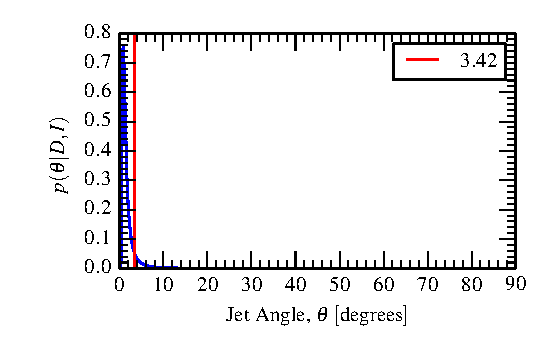
\includegraphics{jet_angle_posterior_s6UL_TEST_deltaEffPrior-1.0.eps}
\caption{$p(\epsilon|I)=\delta(\epsilon-1)$: efficiency assumed known:
$\epsilon=1$}
\end{figure}

\begin{figure}[h!]
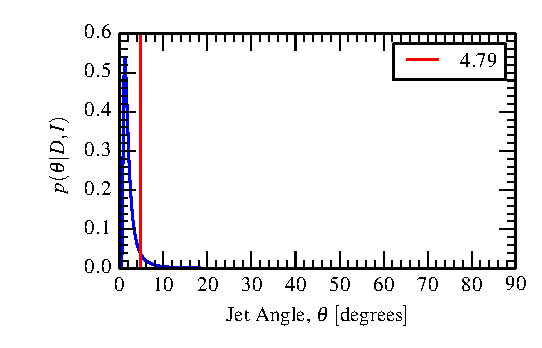
\includegraphics{jet_angle_posterior_s6UL_TEST_deltaEffPrior-0.5.eps}
\caption{$p(\epsilon|I)=\delta(\epsilon-0.5)$: efficiency assumed known:
$\epsilon=0.5$}
\end{figure}

\begin{figure}[h!]
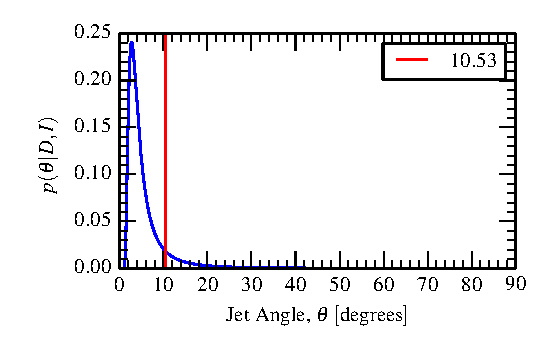
\includegraphics{jet_angle_posterior_s6UL_TEST_deltaEffPrior-0.1.eps}
\caption{$p(\epsilon|I)=\delta(\epsilon-0.1)$: efficiency assumed known:
$\epsilon=0.1$}
\end{figure}

\begin{figure}[h!]
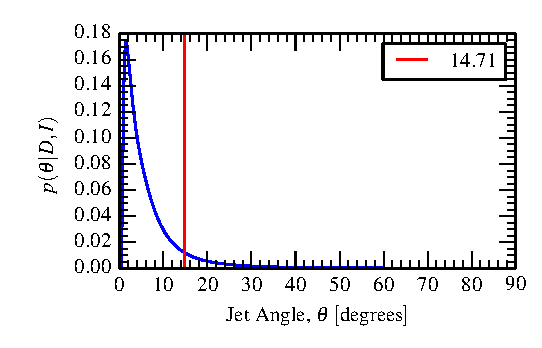
\includegraphics{jet_angle_posterior_s6UL_TEST_flatEffPrior-0.01-1.eps}
\caption{$p(\epsilon|I) \propto 1,~\epsilon \in (0,1]$. 
Here, we assume the GRB efficiency is $\epsilon \in (0,1]$, with no
preference where: the linearly uniform prior.  The reason for choosing a
non-zero lower bound is that the Jacobian determinant goes to $\inf$ as
$\epsilon \rightarrow 0$.  \textcolor{red}{James: I'm very open to suggestions
here as it's not clear to me that this is expected.  In practice, $\epsilon \in
[0.01,1]$}.}
\end{figure}

\begin{figure}[h!]
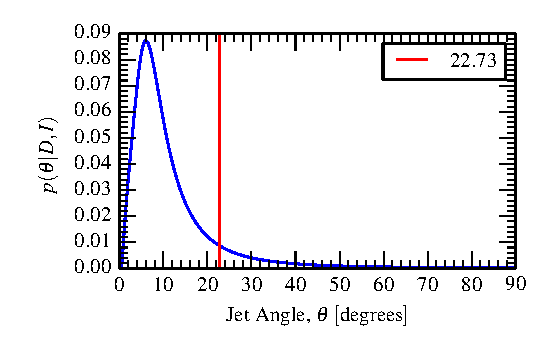
\includegraphics{jet_angle_posterior_s6UL_TEST_logEffPrior-0.01-1.eps}
\caption{$p(\epsilon|I) \propto 1/\epsilon,~\epsilon \in (0,1]$
Now assume the GRB efficiency is $\epsilon \in (0,1]$, with a log-uniform
prior (commonly but incorrectly referred to as the Jeffrey's prior).  Here, the
requirement of a non-zero lower bound is imposed by the normalisation for this
prior.
}
\end{figure}

\begin{figure}[h!]
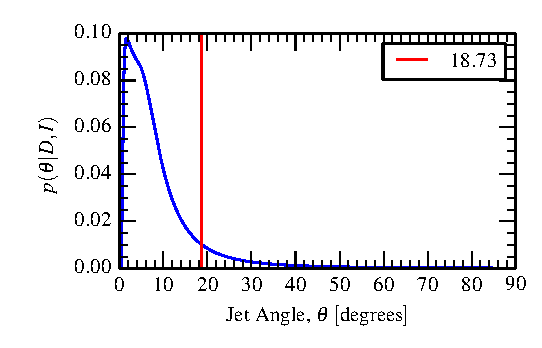
\includegraphics{jet_angle_posterior_s6UL_TEST_bernoEffPrior.eps}
\caption{$p(\epsilon|I) = \beta(1/2,1/2),~\epsilon \in (0,1)$.  Here, we use a
Beta distribution with shape and scale parameters of 1/2.  That prior has a
slightly surprising shape with a minimum at $\epsilon=0.5$ and shoots off to
$\infty$ as $\epsilon\rightarrow 0,1$.  It seems \emph{this} is, in fact, the
Jeffrey's prior for a Bernoulli trial (if we say a toin coss = BNS
$\rightarrow$GRB). See
\href{http://en.wikipedia.org/wiki/Jeffreys_prior}{http://en.wikipedia.org/wiki/Jeffreys\_prior}
}
\end{figure}

\begin{figure}[h!]
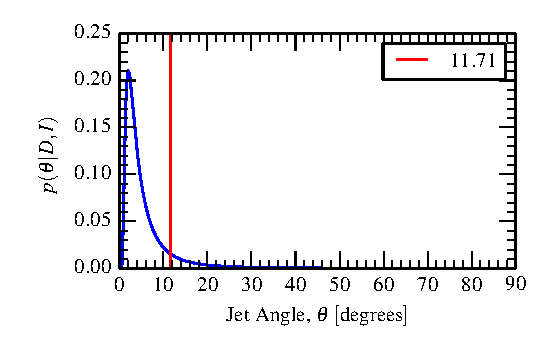
\includegraphics{jet_angle_posterior_s6UL_TEST_betaEffPrior-2-5.eps}
\caption{$p(\epsilon|I) = \beta(2,5),~\epsilon \in (0,1)$.  The GRB efficiency
prior is, this time, a $\beta$ distribution with shape and scale parameters 2
and 5, respectively.  This is now completely ad hoc but yields a maximum (in the
prior) around $\epsilon=0.2$ and goes to 0 as $\epsilon \rightarrow 0,1$.  So
it's a nice example of an asymmetric distribution with quite sensible (and
presumably tuneable) behaviour.}
\end{figure}

\begin{figure}[h!]
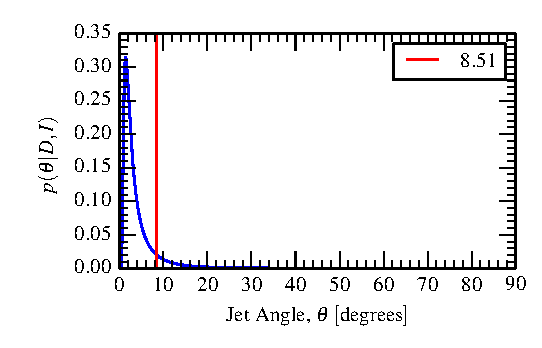
\includegraphics{jet_angle_posterior_s6UL_TEST_betaEffPrior-2-2.eps}
\caption{$p(\epsilon|I) = \beta(2,2),~\epsilon \in (0,1)$.  Finally, we have for
the GRB efficiency prior a $\beta$ distribution with shape and scale parameters 2
and 2, respectively.  Again, this is ad hoc but symmetric about $\epsilon=0.5$
with a cosine-like shape.}
\end{figure}

\bibliography{grb_beams}

\end{document}
